\section{Побудова безхмарного композиту}

Спочатку всі завантажені датасети потрібно очистити від знімків, кожен канал
яких має значення NaN, тобто від зображень чорного кольору.

Потім було прийнято рішення про сортування композитів за відсотком хмарності, інею
та неповних знімків. Цей функціонал було додано в ODC. Неповний знімок --- це
такий самий за розмірністю знімок, як і інші в датасеті, але на ньому відображена не вся
територія. Таким чином відбиралися такі дані, де відсоток загальної хмарності був
не більшим за 35--40 відсотків, оскільки інакше вихідний знімок після роботи алгоритму
буде з дефектами.

На вхід алгоритму, що прибирає хмари, подається множина індексів часу та сам
датасет, з якого беруться ці знімки. На цьому етапі знімки вже пройшли повну попередню обробку і готові
до обробки. Ця процедура (рис. \ref{fig:cloud-removal}) повинна повернути певну
кількість композитів, які потім будуть оброблятися за допомогою медіани.

Для того, щоб проводити вищенаведені операції з великим датасетом, у якому більше
ніж два знімки, було розроблено декілька способів обробки, а саме:

Нехай як вхідний використовується датасет, у якому знімки проіндексовані таким
чином: [1,2,3,4,5,6,...]. Тоді для побудови безхмарного композиту використано
наступні методи комбінування знімків:

\begin{enumerate}
	\item \textbf{Кожний з кожним}. Цей алгоритм полягає у комбінуванні кожного з
		кожним, тобто [1.2],[2.1], але не сам з собою.

		В результаті можна отримати якісне зображення, але з суттєвими затратами комп’ютерних
		ресурсів. На виході буде $n^2 - n$ композитів при $n$ вхідних знімках;

	\item \textbf{Почергова трійка}. На вхід моделі подається почергова трійка, де перший
		знімок буде базовим.

		Приклад: [1,2,3], [2,3,4], [3,4,5].

		Цей метод дає оптимальну якість і є більш ощадливим до обчислювальних
		ресурсів.
\end{enumerate}

Було досліджено швидкодію (рис. \ref{fig:methods-comparison}) кожного з описаних методів комбінування.

З урахуванням отриманих результатів експериментів має сенс надалі використовувати
метод парами ``кожний з кожним'' при відносно малій кількості знімків і ``почергову трійку'',
якщо нас цікавить збереження обчислювальних ресурсів чи часу.

Вихідний знімок був побудований за допомогою методу ``кожний з кожним''.

Для майбутнього покращення якості та швидкості опрацювання великих датасетів
було розглянуто наступні методи комбінування знімків:

\begin{enumerate}
	\item \textbf{Кожний базовий}. На вхід подаються списки виду [1,2,3,4,..], [2,1,3,4,..],
		[3,1,2,4,..],

		Тобто завжди подається весь датасет, причому перший знімок є базовим, а на наступному
		кроці попередній базовий міняється місцями з наступним.

	\item \textbf{Пріоритетність}. Спочатку виконується сортування знімків за
		хмарності у датасеті.

		Нехай є впорядковані знімки [3,2,5,7,6,4,1], тоді 3-ій є базовим. Наступні
		ітерації будуть побудовані таким чином:

		3,2,5,7,6,4

		3,5,7,6,4

		3,7,6,4

		3,4

		Цей метод буде працювати лише тоді, коли базовий знімок має дуже малий відсоток
		хмарності.
\end{enumerate}

Для досягнення найкращої якості вихідного композиту потрібно брати знімки, які є
максимально близькими за часом зйомки. Це забезпечить менший перепад у відтінках
пікселів. Таким чином, після комбінування знімків і заміни захмарених пікселів, маємо
кінцевий масив такого вигляду.

\begin{figure}[H]
	\centering
	\resizebox{!}{1.0\textheight}{%
	\begin{tikzpicture}[
		node distance=7mm and 10mm,
		>=latex',
		every node/.style={font=\small},
		block/.style={ draw, rectangle, line width=0.35pt, minimum height=12mm, minimum width=52mm, text width=48mm, align=center },
		rblock/.style={ draw, rectangle, rounded corners=1em, line width=0.35pt, minimum height=12mm, minimum width=52mm, text width=46mm, align=center },
		cblock/.style={ draw, chamfered rectangle, chamfered rectangle xsep=7mm, line width=0.35pt, minimum height=13mm, minimum width=58mm, text width=52mm, align=center },
		iblock/.style={ draw, trapezium, trapezium left angle=75, trapezium right angle=105, line width=0.35pt, minimum height=12mm, minimum width=52mm, text width=45mm, align=center }
	]
		\node[rblock] (start) {Початок}; \node[block, below=of start] (load-base) {Завантаження\\першого\\композиту\\та маски як\\базових};
		\node[block, below=of load-base] (mask-base)
		{Створюємо маску хмар та\\перистих хмар}; \node[block, below=of mask-base] (dilate-base)
		{Збільшення\\масок}; \node[block, below=of dilate-base] (merge-base)
		{Об'єднуємо маску в одну\\базову};

		\node[cblock, right=18mm of merge-base] (loop-start)
		{Цикл по списку\\композитів починаючи\\з другого}; \node[block, below=of
		loop-start] (load-next) {Завантаження\\наступного\\композиту\\та маски};
		\node[block, below=of load-next] (mask-next)
		{Створюємо маску хмар та\\перистих хмар}; \node[block, below=of mask-next] (dilate-next)
		{Збільшення\\масок}; \node[block, below=of dilate-next] (merge-next)
		{Об'єднуємо маску в одну\\базову}; \node[block, below=of merge-next] (replace)
		{Заміна хмарних пікселів\\по масках}; \node[cblock, below=of replace] (loop-end)
		{Кінець циклу};

		\node[block, left=18mm of loop-end] (median)
		{Застосування\\медіани по\\каналам}; \node[block, below=of median] (restore)
		{Відновлення\\даних}; \node[iblock, below=of restore] (output)
		{Вивід результату}; \node[rblock, below=of output] (end) {Кінець};

		\path[draw, ->] (start) edge (load-base) (load-base) edge (mask-base) (mask-base)
		edge (dilate-base) (dilate-base) edge (merge-base) (merge-base) edge (loop-start)
		(loop-start) edge (load-next) (load-next) edge (mask-next) (mask-next) edge
		(dilate-next) (dilate-next) edge (merge-next) (merge-next) edge (replace) (replace)
		edge (loop-end) (loop-end) edge (median) (median) edge (restore) (restore)
		edge (output) (output) edge (end);
	\end{tikzpicture}%
	}
	\caption{Схема вилучення хмарних пікселів}
	\label{fig:cloud-removal}
\end{figure}

\begin{figure}[H]
	\centering
	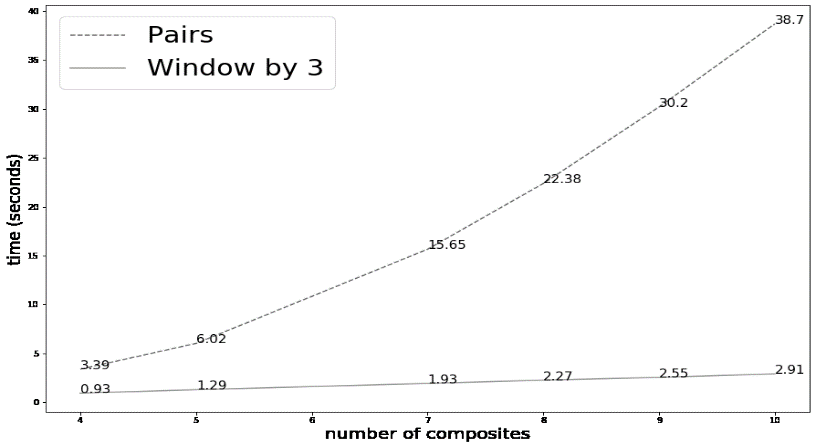
\includegraphics[width=0.7\textwidth]{images/image11}
	\caption{Графік залежності часу від кількості знімків для двох методів
	\label{fig:methods-comparison} }
\end{figure}
